%!TEX root = ../template.tex
%%%%%%%%%%%%%%%%%%%%%%%%%%%%%%%%%%%%%%%%%%%%%%%%%%%%%%%%%%%%%%%%%%%
%% chapter1.tex
%% NOVA thesis document file
%%
%% Chapter with introduction
%%%%%%%%%%%%%%%%%%%%%%%%%%%%%%%%%%%%%%%%%%%%%%%%%%%%%%%%%%%%%%%%%%%

\typeout{NT FILE chapter1.tex}%

\chapter{Introduction}
\label{cha:Introduction}

\prependtographicspath{{Chapters/Figures/Covers/}}


\section{Motivation}
\label{sec:Motivation}

The ever-growing demand for efficient and accurate DNA sequencing solutions has highlighted the limitations of traditional methods, particularly in high-throughput environments. Sanger sequencing remains a widely used technique due to its reliability and precision. However, the manual verification of alignment results introduces bottlenecks that hinder the scalability and efficiency of laboratories, especially those handling extensive genomic datasets.

This bottleneck is not merely an operational issue but a scientific challenge. As genomic research expands its applications in fields like medicine, agriculture, and biotechnology, the need for automated tools capable of minimizing errors and optimizing workflows becomes increasingly evident. By integrating artificial intelligence (AI) into these processes, laboratories can achieve new levels of efficiency and accuracy, ultimately advancing the frontiers of genomic research.

\section{Context}
\label{sec:Context}

\subsection{Introduction to DNA}
DNA (deoxyribonucleic acid) is the molecular blueprint for all living organisms, carrying the genetic instructions necessary for growth, development, and reproduction. The structure of DNA was famously elucidated by Watson and Crick in 1953, a discovery that revolutionized molecular biology \cite{watson_crick_dna}. DNA consists of two complementary strands coiled into a double helix, with nucleotide bases (adenine, thymine, cytosine, and guanine) forming the rungs of the helix \cite{khan_dna_structure}.

\begin{figure}[H]
\centering
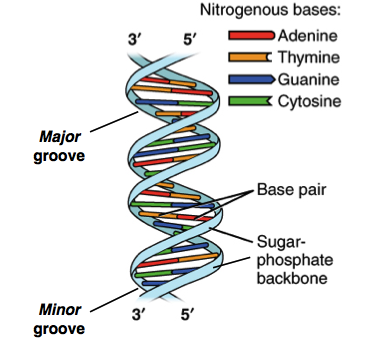
\includegraphics[width=0.5\textwidth]{dna_double_helix.png}
\caption{The structure of the DNA double helix.}
\label{fig:dna_double_helix}
\end{figure}

\subsection{DNA Sequencing and Sanger Sequencing}
DNA sequencing is the process of determining the precise order of nucleotides within a DNA molecule. Among the various sequencing methods, Sanger sequencing remains a widely utilized technique due to its accuracy and reliability. Developed by Frederick Sanger and colleagues in 1977, this method involves the selective incorporation of chain-terminating dideoxynucleotides (ddNTPs) by DNA polymerase during in vitro DNA replication \cite{sanger_method_original}.

Sequencing DNA is fundamental to understanding genetic information, enabling applications ranging from disease diagnosis and treatment to evolutionary biology \cite{turn0search0}. By deciphering the nucleotide order, scientists can identify mutations, study gene expression, and uncover genetic diversity.

The steps of Sanger sequencing are enumerated as follows and illustrated in Figure \ref{fig:sanger_steps}: 
\begin{enumerate} 
\item \textbf{Primer annealing and chain extension}: DNA polymerase synthesizes complementary DNA strands using a primer and a mixture of deoxynucleotides (dNTPs). 
\item \textbf{ddNTP binding and chain termination}: The incorporation of ddNTPs halts DNA synthesis at specific nucleotides, resulting in DNA fragments of varying lengths. 
\item \textbf{Fluorescent labeling of DNA fragments}: The terminated DNA strands are fluorescently labeled for detection. 
\item \textbf{Capillary gel electrophoresis and fluorescence detection}: DNA fragments are separated by capillary gel electrophoresis and identified based on fluorescence signals. 
\item \textbf{Sequence analysis and reconstruction}: The nucleotide sequence is reconstructed from the fluorescence data and analyzed. 
\end{enumerate}

\begin{figure}[H]
\centering
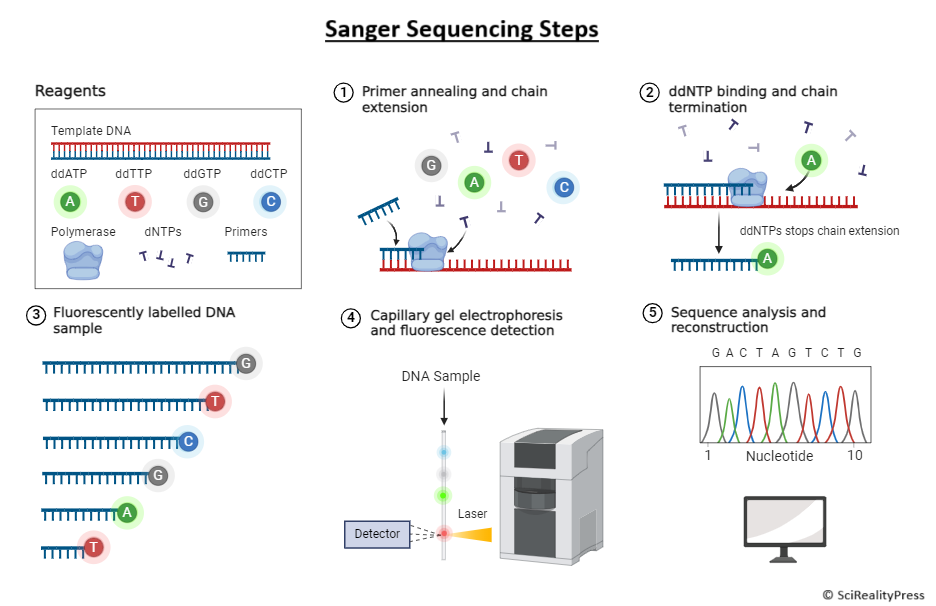
\includegraphics[width=0.8\textwidth]{sanger_steps.png}
\caption{Steps involved in Sanger sequencing \cite{biotechreality_sanger_steps}.}
\label{fig:sanger_steps}
\end{figure}

To better understand the components involved in this process:
\begin{itemize}
    \item \textbf{DNA Template}: The single-stranded DNA to be sequenced.
    \item \textbf{Primer}: A short single-stranded oligonucleotide complementary to the target sequence, serving as the starting point for DNA synthesis.
    \item \textbf{DNA Polymerase}: An enzyme that synthesizes new DNA strands by adding nucleotides to the primer.
    \item \textbf{Deoxynucleotides (dNTPs)}: Normal nucleotides (A, T, C, G) used to elongate the DNA strand.
    \item \textbf{Dideoxynucleotides (ddNTPs)}: Modified nucleotides (ddATP, ddTTP, ddCTP, ddGTP) that terminate DNA strand synthesis upon incorporation due to the lack of a 3′-OH group.
\end{itemize}

\subsection{The ABI3730xl DNA Sequencer}
The ABI3730xl DNA sequencer is a high-throughput instrument widely used in genomics for Sanger sequencing. It automates the electrophoresis and fluorescence detection steps, corresponding to steps 3 and 4 of the Sanger sequencing process (Figure \ref{fig:sanger_steps}), allowing for the simultaneous processing of 96 samples in a single run \cite{smith_capillary_sequencing,abi3730xl_overview}. By leveraging this technology, laboratories can achieve precise and efficient DNA sequencing. 
\begin{figure}[h]
\centering
\includegraphics[width=0.7\textwidth]{abi_3730xl_closed.png}
\caption{A closed ABI3730xl capillary electrophoresis DNA analyzer.}
\label{fig:abi_3730xl_closed}
\end{figure}

\begin{figure}[h]
\centering
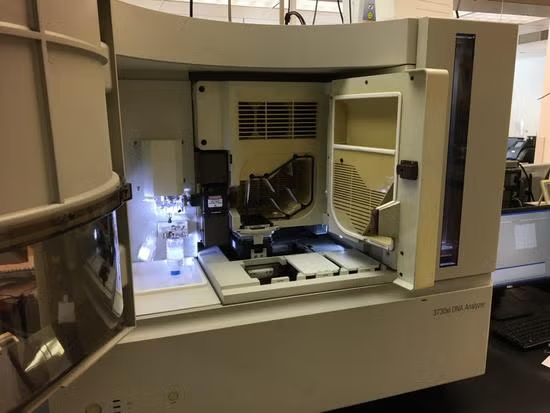
\includegraphics[width=0.7\textwidth]{abi_3730xl_opened.png}
\caption{A opened ABI3730xl capillary electrophoresis DNA analyzer.}
\label{fig:abi_3730xl_opened}
\end{figure}


\subsection{Role of Artificial Intelligence in DNA Analysis}
Artificial intelligence (AI) revolutionizes genomic research by enhancing the accuracy and efficiency of data analysis. Machine learning (ML) models, trained on extensive genomic datasets, excel at recognizing patterns and anomalies. In Sanger sequencing, AI can:
\begin{itemize}
\item Detect mislabeled or erroneous sequences.
\item Automate anomaly identification in 96-well plate outputs.
\item Reduce human intervention while improving data reliability.
\end{itemize}

Ethical considerations must accompany AI integration to safeguard data privacy, address biases, and ensure equitable access to technology. The synergy between AI and DNA sequencing promises advancements in precision medicine and genomics.

\subsection{Machine Learning and Deep Learning in Genomics}
Machine Learning (ML) and Deep Learning (DL) are subfields of Artificial Intelligence (AI) that have revolutionized various scientific disciplines, including genomics, in which both of these fields have transformed the landscape of genomic research \cite{ml_genomics_review}. These computational approaches enable systems to learn patterns and make predictions based on large datasets, bypassing the need for explicitly programmed instructions.
ML algorithms, such as support vector machines and random forests, excel in identifying patterns within large datasets, while DL models, like convolutional neural networks (CNNs), are adept at analyzing complex, high-dimensional data \cite{libbrecht_ml_genomics,dl_methods_genomics}.

\paragraph{Machine Learning:}
ML refers to algorithms that improve their performance on a task with experience. In the context of DNA sequencing:
\begin{itemize}
\item Supervised learning algorithms are trained using labeled datasets, such as annotated DNA sequences, to classify or predict sequence anomalies.
\item Unsupervised learning algorithms, like clustering methods, identify patterns in unlabeled data, such as grouping similar DNA sequences.
\item Reinforcement learning methods optimize decision-making processes, like adjusting sequencing parameters for improved accuracy.
\end{itemize}

\paragraph{Deep Learning:}
DL, a subset of ML, uses artificial neural networks inspired by the human brain. These networks, especially when designed as deep architectures, are particularly effective in handling large and complex datasets such as genomic data. In Sanger sequencing:
\begin{itemize}
\item Convolutional Neural Networks (CNNs) can process visual data from electropherograms to identify signal anomalies.
\item Recurrent Neural Networks (RNNs) or their advanced variants (e.g., Long Short-Term Memory networks, LSTMs) are ideal for analyzing sequential data, such as nucleotide chains.
\item Autoencoders and Generative Adversarial Networks (GANs) are employed for noise reduction and synthetic data generation, enhancing training datasets.
\end{itemize}

In genomics, these techniques are employed for tasks such as sequence alignment, variant calling, and the identification of genetic mutations \cite{ml_dna_applications}. The integration of AI into Sanger sequencing workflows, as in this thesis, enables the automation of error detection and data validation, enhancing the accuracy and efficiency of sequencing processes \cite{ai_sanger_sequencing,esteva_ai_genomics}.

\paragraph{Applications in Sanger Sequencing:}
Integrating ML and DL into Sanger sequencing workflows enables:
\begin{itemize}
\item Automated classification of sequencing errors, such as those caused by fluorescent signal overlap or ddNTP misincorporation.
\item Enhanced post-sequencing analysis to flag inaccurate well outputs in 96-well plates.
\item Streamlined data analysis pipelines, reducing the time and labor required for manual verification.
\end{itemize}

The combination of these AI-driven methodologies with established sequencing technologies, such as the ABI3730xl, provides a robust framework for addressing critical challenges in genomic research. It bridges the gap between raw sequencing data and actionable biological insights, reinforcing the importance of interdisciplinary approaches in modern science.
  
\subsection{Broader Scientific Implications}
Studying DNA and developing advanced sequencing tools contribute to:
\begin{itemize}
\item \textbf{Precision Medicine}: Personalizing treatments based on genetic profiles.
\item \textbf{Evolutionary Biology}: Understanding species evolution and genetic diversity.
\item \textbf{Agriculture}: Enhancing crop yields and pest resistance through genetic insights.
\item \textbf{Biotechnology}: Innovating in synthetic biology and gene editing applications.
\end{itemize}

Through the combination of traditional techniques, cutting-edge sequencing technologies, and AI, this thesis addresses the critical challenge of post-sequencing analysis, pushing the boundaries of what is possible in modern genomics.

\section{Objectives}
\label{sec:Objectives}

The primary goal of this thesis is to develop a tool that automates the verification of alignment results obtained from Sanger sequencing. The specific objectives include:

\begin{itemize}
  \item Designing an AI algorithm capable of detecting anomalies and homologous sequences in alignment data.
  \item Training the algorithm using real-world datasets from ABI3730xl sequencers 96-well plates.
  \item Designing an AI algorithm capable of detecting anomalies and homologous sequences in alignment data.
  \item Training the algorithm using real-world datasets from ABI3730xl sequencers 96-well plates.
  \item Validating the tools performance against traditional manual verification methods.
  \item Deploying the tool via an online platform to ensure accessibility for laboratories worldwide.
\end{itemize}

\section{Structure}
\label{sec:Structure}

This document is organized as follows:

\begin{itemize}
  \item Introduction: Provides the motivation, context, objectives, and structure of the thesis.
  \item State of the Art \& Related Work: Reviews existing literature and technologies in Sanger sequencing and AI applications in genomics.
  \item Methodology: Details the design and implementation of the proposed AI driven tool, including data collection, model training, and deployment.
  \item Planning: Presents the planning of the proposed work, composed by desired checkpoints and finish dates.
  \end{itemize}
% subsection suggestions_bugs_and_feature_requests (end)
